% CSE Seminararbeit
% Thema: Ein auf Neuronalen Netzen basierendes Ensemble-Modell zur Windprognose
% Autoren: Alicia Pirwass, Daniel Müller

\documentclass[
12pt, %Schriftgröße
toc=listofnumbered, %Tab.- & Abb.verzeichnis ins TOC
toc=chapterentrydotfill, %TOC: Punkte auch nach Kapitel
numbers=noenddot, %Kapitelüberschrift: Kein Endpunkt z.B. 2.2. --> 2.2
captions=tableheading, %Mehr Platz bei Captionüberschriften (Tabelle)
bibliography=numbered
]{scrreprt}


%%%%% SCHRIFTSATZ, SPRACHE, SCHRIFTART
%%% USE WITH pdflatex, siehe https://tex.stackexchange.com/a/44701
%\usepackage[T1]{fontenc}
%\usepackage[utf8]{inputenc}
%%% USE WITH xelatex
\usepackage{fontspec}
\defaultfontfeatures{Ligatures=TeX}
%%% USE WITH lualatex
%\usepackage{luatextra}
%\defaultfontfeatures{Ligatures=TeX}
%%%
\usepackage[ngerman]{babel}
% Nur mit LuaTex Interpreter nutzbar
%\usepackage{mathfont} % Dieses Packet läd auch fontspec
%\setmainfont{Segoe Pro} % Textschrift separat setzen


%%%%% INHALTSVERZEICHNIS
%\setuptoc{toc}{numbered} % TOC ins TOC, benötigen wir hier nicht 
%\addtokomafont{chapterentrypagenumber}{\normalfont\textbf}

\addtokomafont{disposition}{\rmfamily}
\addtokomafont{chapterentry}{\textbf}
\RedeclareSectionCommand[tocnumwidth=2.5em]{chapter}
\RedeclareSectionCommand[tocnumwidth=2.5em,tocindent=2.5em]{section}
\RedeclareSectionCommand[tocnumwidth=2.5em,tocindent=5em]{subsection}
%\newcounter{romanchapter} Benötigen wir nur, wenn z.B. Abstract, Literaturverz. und Anhang römisch nummeriert werden soll


%%%%% MATHEMATIK
\usepackage{amssymb, amsmath}
\usepackage{isomath}
\usepackage{pifont} % Für \cmark und \xmark
\newcommand{\cmark}{\ding{51}}%
\newcommand{\xmark}{\ding{55}}%


%%%%% BIBLIOGRAPHIE
\usepackage[style=ieee, mincitenames=1, maxcitenames=1]{biblatex}
\usepackage{url} % Damit URLs in der Quelle schön umgebrochen werden
\setcounter{biburllcpenalty}{7000} % Einstellungen für Packet url
\setcounter{biburlucpenalty}{8000} % Einstellungen für Packet url
\DefineBibliographyStrings{ngerman}{andothers = {{et\,al\adddot}},}
\addbibresource{bib.bib} %
\usepackage{csquotes}
%\emergencystretch=1em
\usepackage[final]{microtype}
%\usepackage[expansion, final]{microtype}
%\usepackage{natbib}
%\setcounter{biburlnumpenalty}{9000}
%\setcounter{biburllcpenalty}{9000}
%\setcounter{biburlucpenalty}{9000}


%%%%% ANHANG
\usepackage{appendix}


%%%%% FARBEN
\usepackage[table,xcdraw]{xcolor}
\definecolor{color20}{RGB}{35,35,35}
\definecolor{color25}{RGB}{69,69,69}
\definecolor{color30}{RGB}{80,80,80}
\definecolor{color80}{RGB}{190,190,190}


%%%%% ÜBERSCHRIFTEN DER EBENEN ÄNDERN
\addtokomafont{chapter}{\color{color30}\normalfont\textbf}
\addtokomafont{section}{\color{color30}\normalfont\textbf}
\addtokomafont{subsection}{\color{color30}\normalfont\textbf}
\addtokomafont{caption}{\small\color{color30}\textit}
\addtokomafont{captionlabel}{\small\color{color30}\textit}


%%%%% LAYOUT
\usepackage[left=2cm,right=2cm,top=3cm,bottom=3cm]{geometry}
\setlength\parindent{0pt} %Kein Einzug nach Ebenenbeginn
\usepackage[onehalfspacing]{setspace} %Zeilenabstand 1,5
\RedeclareSectionCommand[beforeskip=20pt,afterskip=20pt]{chapter} %Wenn neues Chapter startet, geht es auf ne neue Seite. Damit Abstand zur Kopfzeile nicht zu groß, beforeskip = 20
\usepackage[justification=justified,labelfont=bf,format = plain]{caption}


%%%%% KOPF- & FUẞZEILE
\usepackage[headsepline,automark]{scrlayer-scrpage}
\pagestyle{scrheadings}
\clearscrheadfoot
\clearscrplain 
\ihead{\headmark}
\ofoot{\pagemark}
\renewcommand*\chapterpagestyle{scrheadings} %K.&F.zeile auch bei Chapterbeg.


%%%%% BILDER
\usepackage{graphicx}
\usepackage[export]{adjustbox}
\usepackage[section]{placeins}
\let\Oldsection\section
\renewcommand{\section}{\FloatBarrier\Oldsection}
\let\Oldsubsection\subsection
\renewcommand{\subsection}{\FloatBarrier\Oldsubsection}
\let\Oldsubsubsection\subsubsection
\renewcommand{\subsubsection}{\FloatBarrier\Oldsubsubsection}
%\usepackage{here} % mit H in includegrafix wird Bildpos gezwungen


%%%%% TABELLE
\usepackage{multirow}
\usepackage{tabularx} % Nachfolgende 3 Befehle, damit Tabellen Spaltengröße definiert werden kann. z.B. nicht mehr {ccc} sondern {C{2cm}C{2cm}C{2cm}}, Folgende befehle zur neu Definition:
\newcolumntype{L}[1]{>{\raggedright\arraybackslash}p{#1}}
\newcolumntype{C}[1]{>{\centering\arraybackslash}p{#1}}
\newcolumntype{R}[1]{>{\raggedleft\arraybackslash}p{#1}}
\usepackage{longtable} %Mehrseitige Tabellen (Abkürzungsverz.)
\setlength{\tabcolsep}{0.5em} % for the horizontal padding
\renewcommand{\arraystretch}{1.2}% for the vertical padding


%%%%% QUICK COMMANDS
\newcommand{\qm}[1]{\glqq#1\grqq{}} %Anfzeichen
\newcommand{\gradC}[1]{#1$^\circ C$}
\newcommand{\abs}[1]{\lvert #1 \rvert}
\newcommand{\highlight}[1]{\textbf{\textcolor{red}{#1}}}
\newcommand{\finalize}[1]{\textcolor{red}{#1}}
\newcommand{\Abb}[1]{\autoref{fig:#1}}

%%%%% VERLINKUNG
\usepackage[hidelinks,hypertexnames=false]{hyperref}
\hypersetup{pdftitle={CSE Projektarbeit, Pirwass und Müller}}

\begin{document}
\begin{titlepage}
    \begin{center}
		%%%%%DOPPELBILD ANFANG
		\begin{minipage}[b]{\linewidth}
			\centering
			\begin{minipage}[b]{.4\linewidth}
				
\includegraphics[width=.8\linewidth, left]{./images/logo_uu.png}
			\end{minipage}
			\hspace{.1\linewidth}% Abstand zwischen Bilder
			\begin{minipage}[b]{.4\linewidth}
				
\includegraphics[width=.6\linewidth, right]{./images/logo_thu.png}
			\end{minipage}
		\end{minipage}
		%%%%%DOPPELBILD ENDE
        
		\vspace{3cm}

        \Huge
		\textbf{Windprognose mit neuronalen Netzen}
            
        \vspace{1.5cm}
        \large
        \textbf{Seminararbeit im Kooperationsstudiengang}\\
		\textbf{Computational Science and Engineering Master}
    \end{center}        
	\vfill
	\large	
	\textbf{Erstellt von:}

	Daniel Müller (1085380)\\
	Alicia Pirwass (1085100)

	\vspace{1cm}
	\textbf{Unter der Leitung von:}

	Professor Dr. Stephan Schlüter

	\vspace{1cm}
	\textbf{Abgabedatum:}

	

	\today
            
    
\end{titlepage}
\tableofcontents
%%%%%%%%%%%%%%%%%%%%%%%%%%%%%%%%%%%%%%%%%%%%%%%%%%%%%%%%%%%%%%%%%%%%%%%
%                                                                     %
%                                                                     %
%                                                                     %
%                               KAPITEL                               %
%                                                                     %
%                                                                     %
%                                                                     %
%%%%%%%%%%%%%%%%%%%%%%%%%%%%%%%%%%%%%%%%%%%%%%%%%%%%%%%%%%%%%%%%%%%%%%%
\chapter{Einleitung}

Die Windenergie leistete in den vergangen Jahren einen stetig wachsenden Beitrag zur deutschen Stromerzeugung. 
Seit dem Jahr 2015 "ist die Stromerzeugung aus Wind [...] um mehr als 60 Prozent angestiegen" \highlight{Quelle Umweltbundesamt, hilfe wie kann ich hier Gänsefüßchen machen?}
Laut dem Statistischen Bundesamt wurden im Jahr 2020 24\% des Gesamtstrommixes in Deutschland aus Windenergie gewonnen. \highlight{vgl. Bild von Strommix} 
Das macht den größten Anteil der erneuerbaren Energien aus \highlight{vgl. Umweltbundesamt}
Jedoch ist das Stromnetz zu veraltet um mit diesen Entwicklungen, hauptsächlich den leistungsstarken Windparks auf See, 
mithalten zu können. Die Netze .. gelangen an die Grenzen ihrer Übertragungskapazität .. \highlight{Quelle windenergie.de}. 
Um diesen Netzengpässen entgegenzuwirken können neben der Erneuerung des Netzes und der Regelung erneuerbarer Erzeugungsanlagen 
des Betreibers Netzoptimierungsmaßnahmen durchgeführt werden. Hierbei wird versucht das bestehende Netz effizient zu nutzen. 
Eine möglicher Ansatz der Netzoptimierung ist das Freileitungsmonitoring. 
Durch eine Überwachung der Windgeschwindigkeit und der Umgebungstemperatur kann daraus die zulässige Übertragungskapazität ermittelt werden. 
Leiterseile halten bei hoher Windgeschwindigkeit und gleichzeitig niedrigen Temperaturen höhere Belastungen aus. 
Es kann also mehr Strom übertragen, wen mehr Windstrom erzeugt wird.\highlight{vgl Quelle windenergie.de}
Aus diesem Grund ist es von großem Interesse Vorhersagen über die Windgeschwindigkeit treffen zu können, um 
die Nutzung des Stromnetzes zu optimieren. In dieser Seminararbeit soll ein Modell entwickelt werden, das 
Windgeschwindigkeit und -richtung eine bis 24 Stunden im Voraus vorhersagen kann.


%%%%%BILD ANFANG
\begin{figure}[tph]
	\begin{center}
		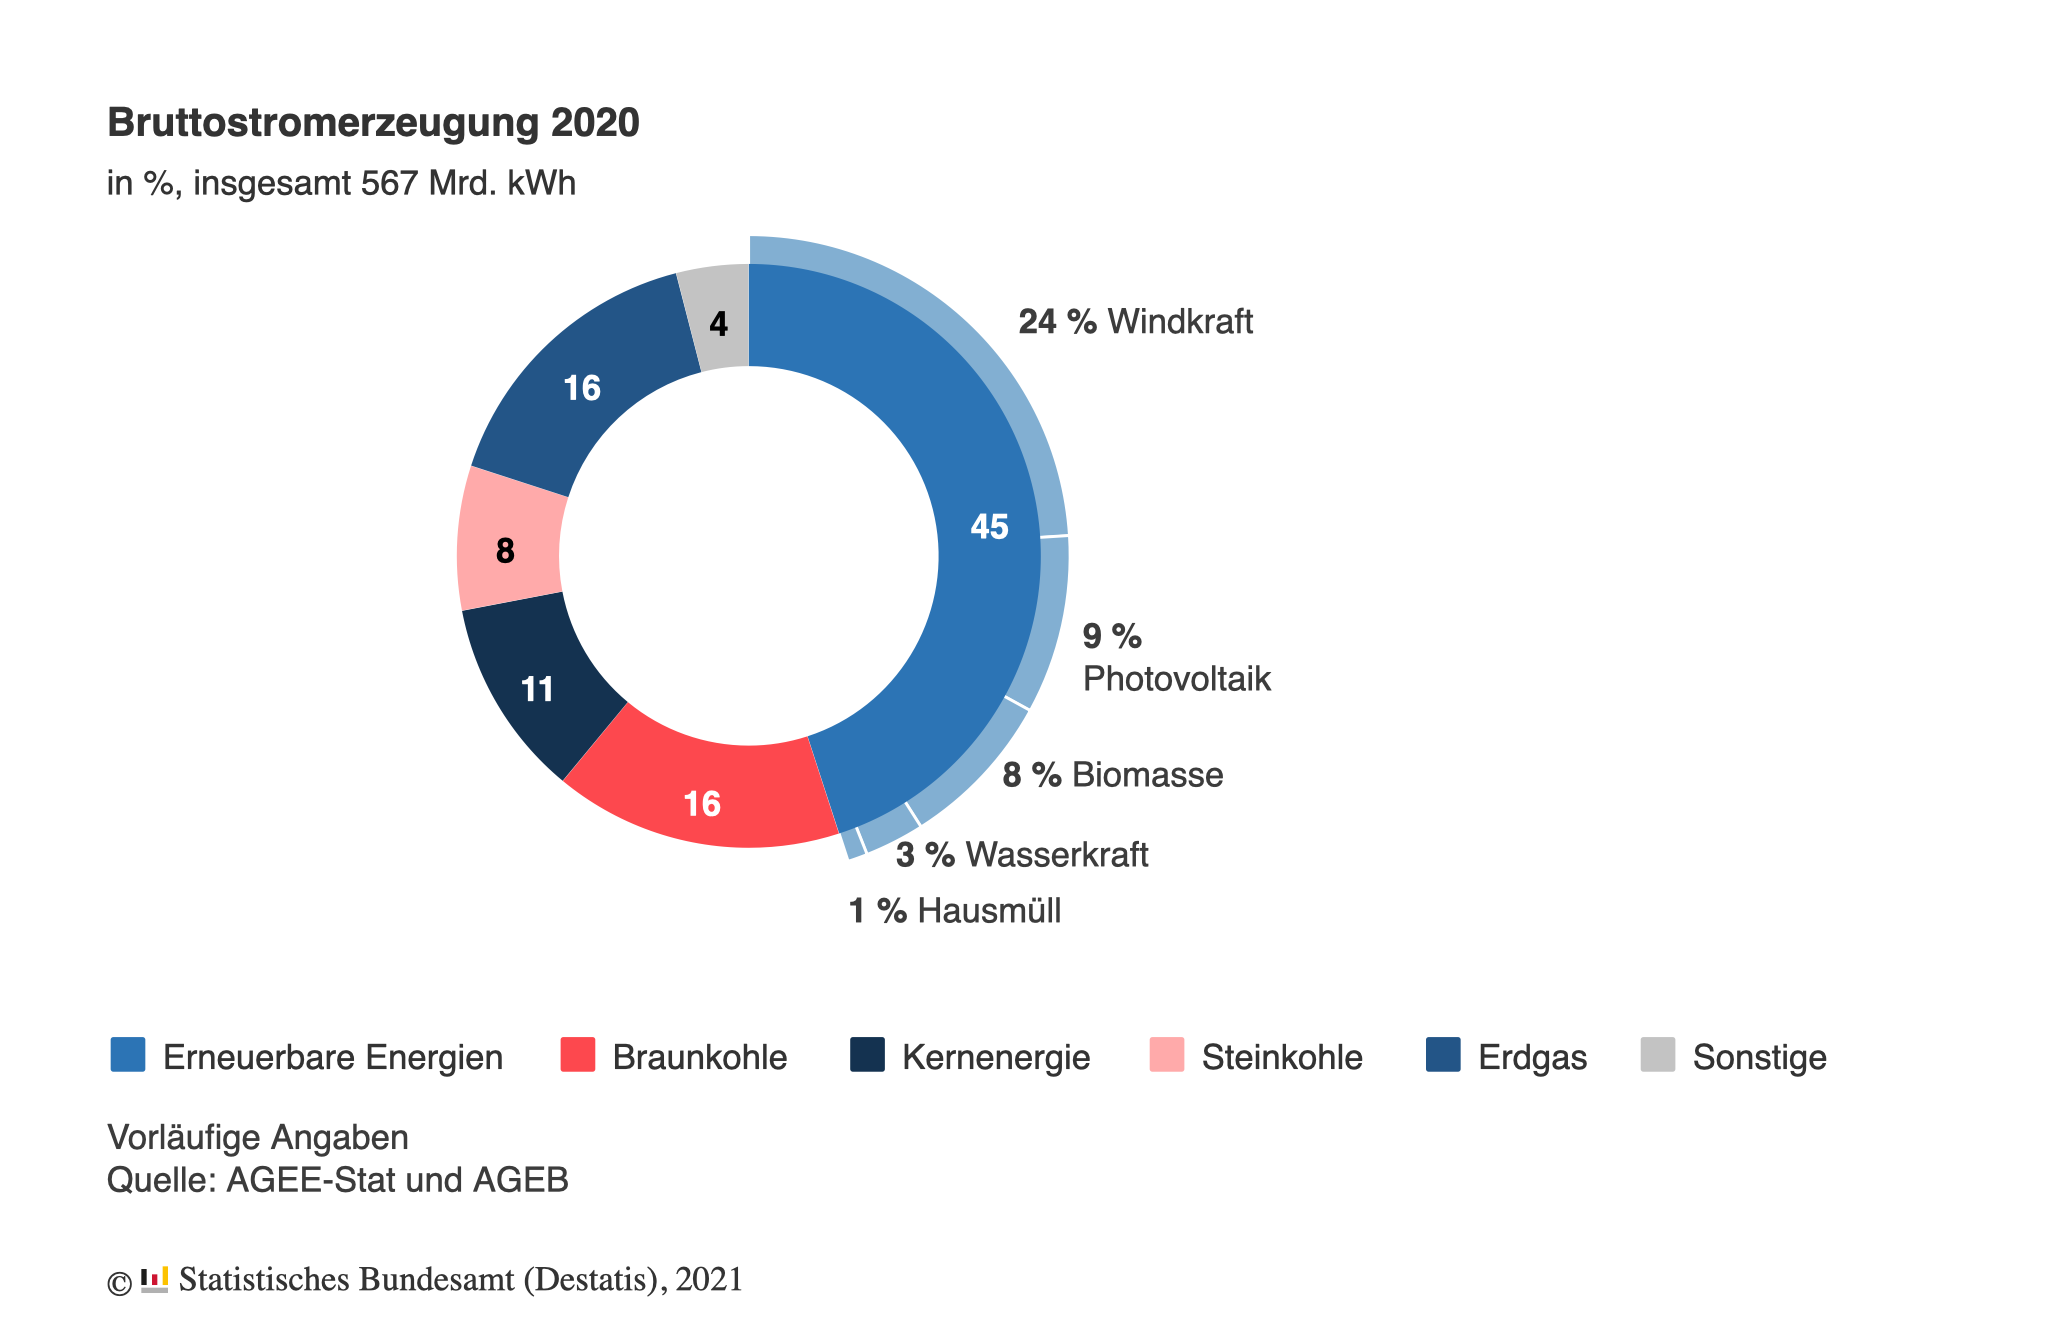
\includegraphics[width=.8\textwidth]{./images/bruttostromerzeugung-erneuerbare-energien.png}
		\caption{Bruttostromerzeugung im Jahr 2020 in Deutschland}
		\label{fig:strommix_deutschland}
	\end{center}
\end{figure}
%%%%%BILD ENDE

\highlight{Sehr gute einleitende Graphiken zur aktuellen Lage der Windkraft in Deutschland, Bilder lassen sich als PDF runterladen!\\
https://www.wind-energie.de/themen/zahlen-und-fakten/deutschland/}

\highlight{Erklären was das besondere an dieser Arbeit ist: 1 Standort wird mit 3 weiteren Standorten prognostiziert}


%%%%%BILD ANFANG
\begin{figure}[tph]
	\begin{center}
		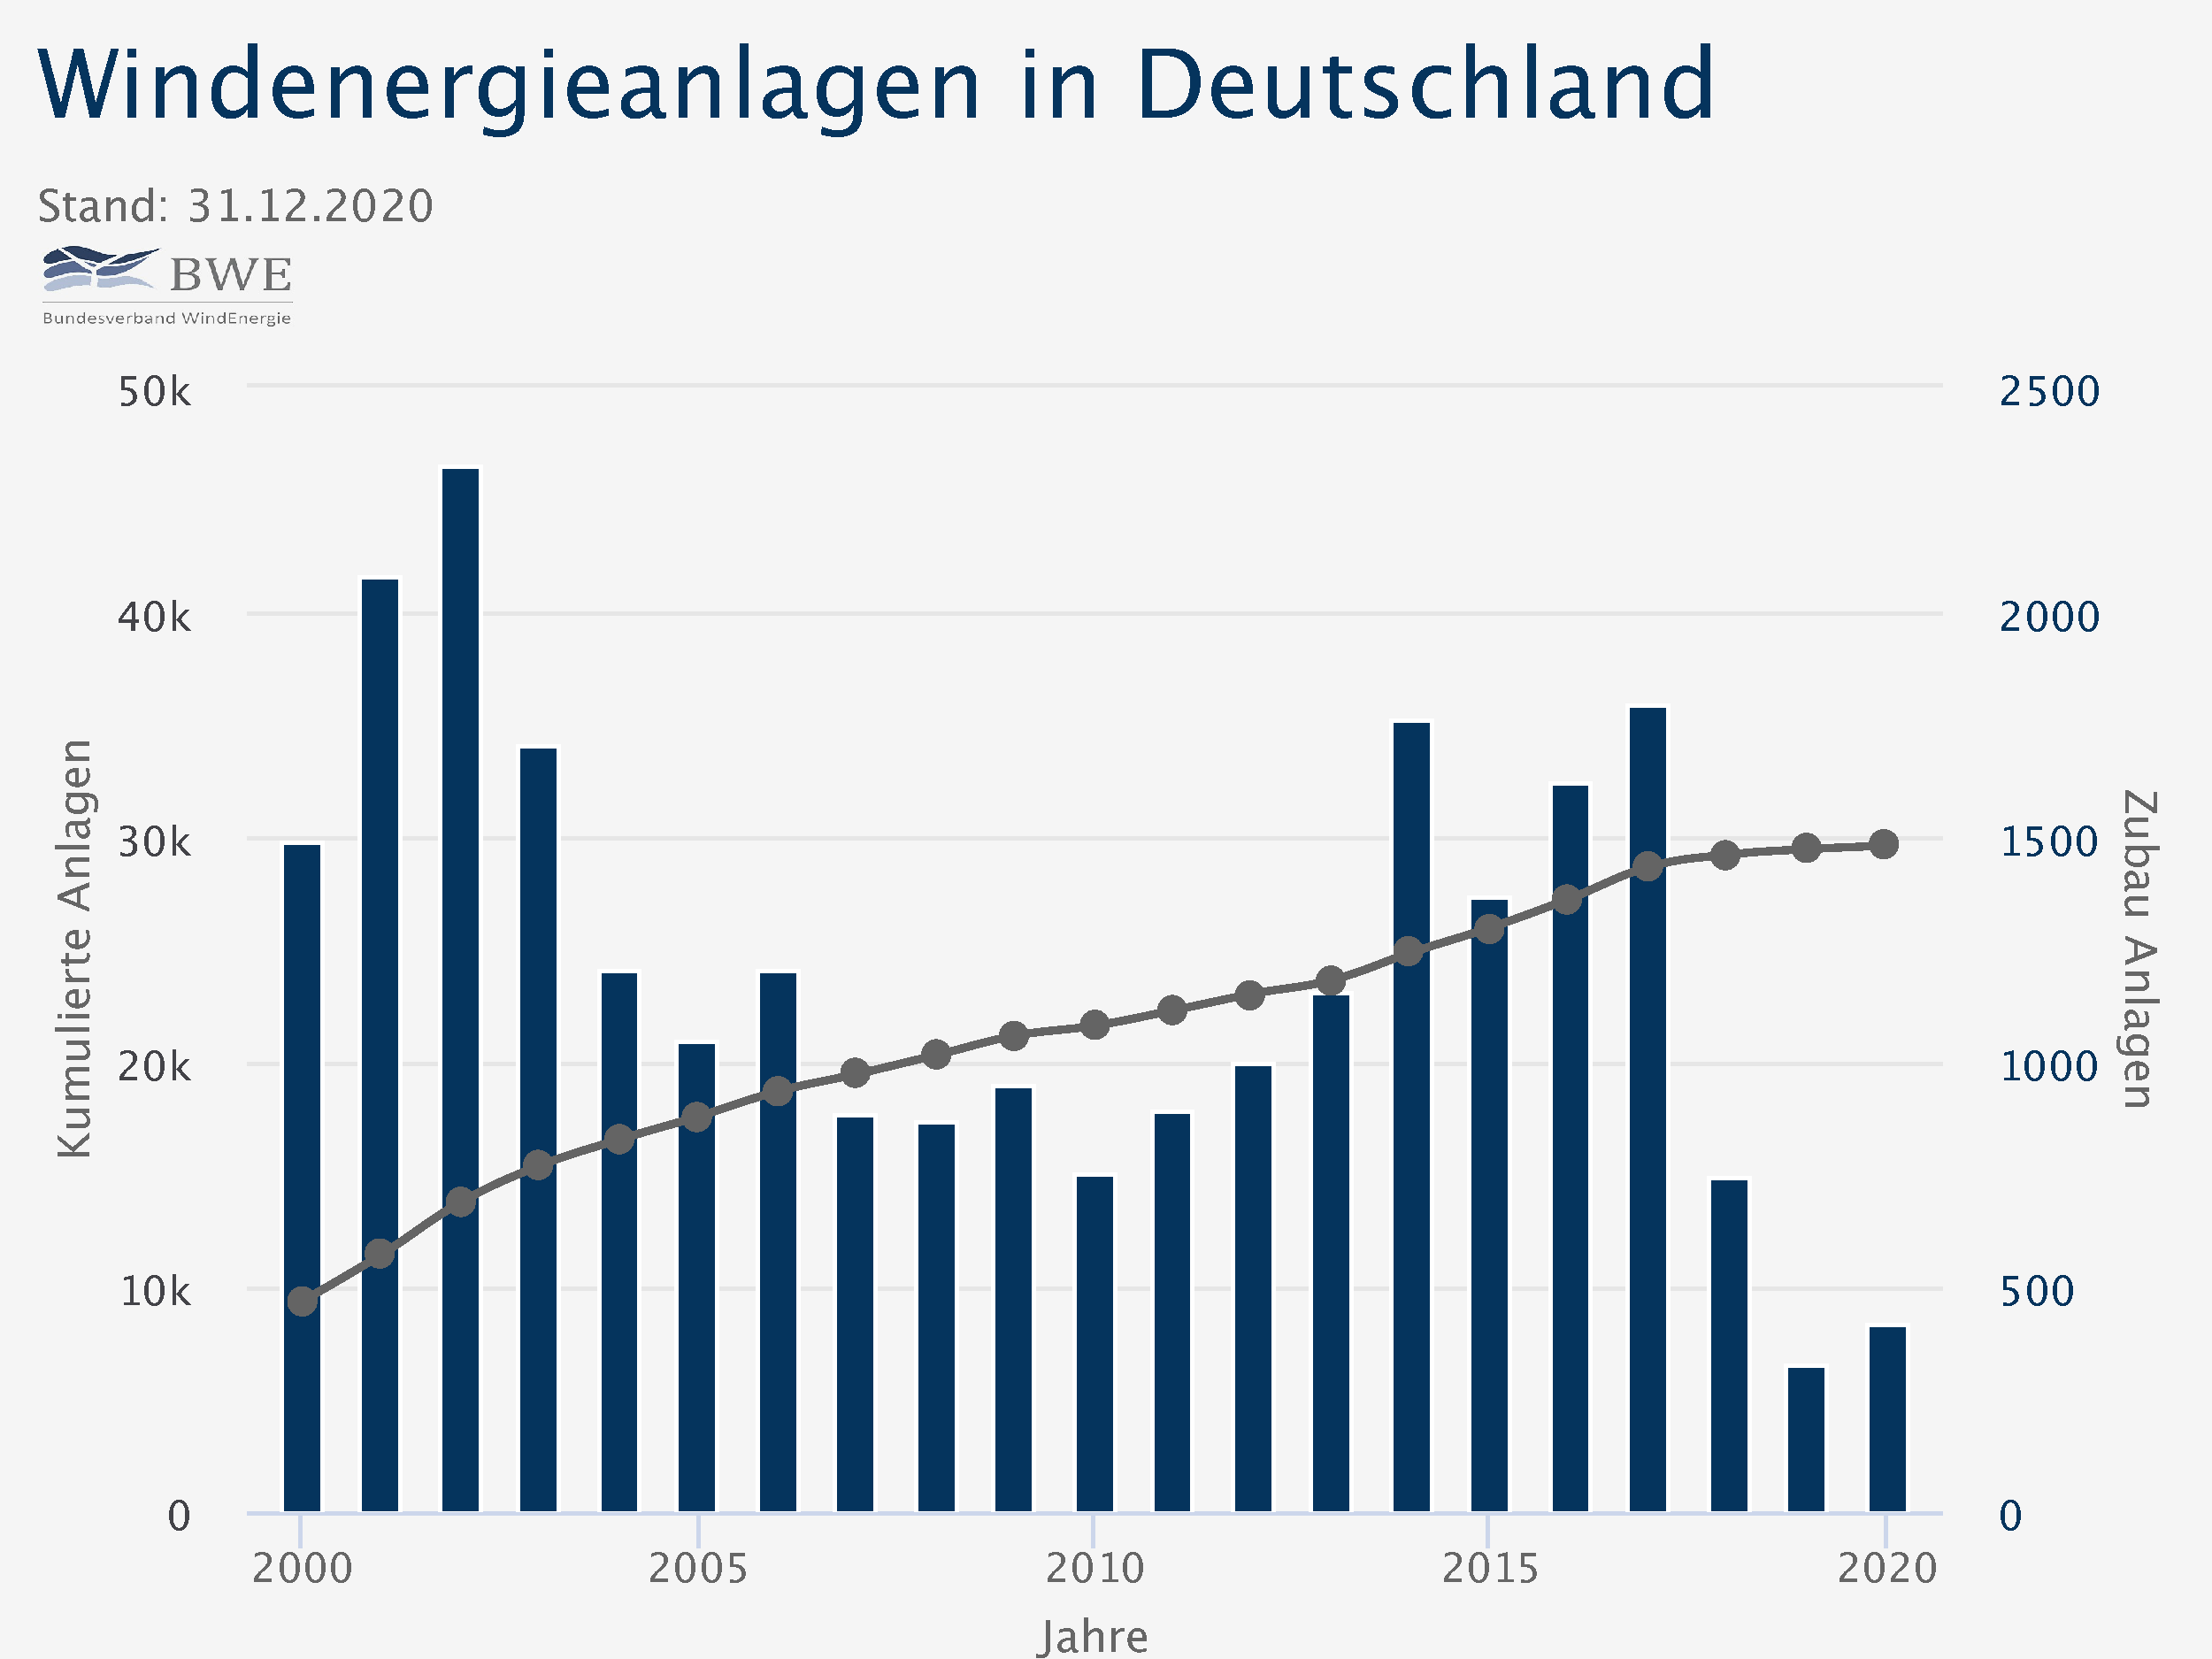
\includegraphics[width=.8\textwidth]{./images/windanlagen_deutschland.pdf}
		\caption{Aktueller Stand der Windkraft in Deutschland; Massiver Rückgang im Zubau in den letzten drei Jahren. \highlight{https://www.wind-energie.de/themen/zahlen-und-fakten/deutschland/ am 19.03.2021}}
		\label{fig:windkraft_deutschland}
	\end{center}
\end{figure}
%%%%%BILD ENDE

\section{Ziel dieser Arbeit}
\highlight{soll in Einordnung in Literatur einfließen. Das wäre zu wenig Inhalt für einen Abschnitt.}

\section{Einordnung in die Literatur}
\highlight{@Alicia: Paper \qm{Multifactor spatio-temporal correlation model based on a combination of convolutional neural network and long short-term memory neural network for wind speed forecasting} in Quelle \cite{2019_Chen_MultifactorSpatiotemporalCorrelation}\bigskip}

In der bestehenden Literatur im Bereich der Windgeschwindigkeits-, beziehungsweise Wettervorhersage, ist eine Entfernung von 
deterministischen Modellen \cite{1963_Lorenz_DeterministicNonperiodicFlow} hin zu Zeitreihenanalyse auf Basis historischer Messdaten erkennbar. 
Innerhalb der letzten zwei Dekaden sind einige Ansätze in der Zeitreihenanalyse zu differenzieren. Klassische Methoden in der 
Zeitreihenprognose, wie das ARMA- und ARIMA-Modell \cite{2016_Cadenas_WindSpeedPrediction} oder auch 
die Weiterentwicklung dessen, mit Berücksichtigung eines saisonalen Einflusses, das SARIMA-Modell 
\highlight{Es fehlt noch Meng 2010; Im Ordner Literatur}\cite{2018_Alencar_HybridApproachCombining,2019_TenaGarcia_ForecastDailyOutput,2019_Haddad_WindSolarForecasting,2002_Igboekwe_StochasticSimulationHourly,2012_MuhammadSami_PredictionRateDust} sind 
nicht nur ein häufig verwendetes Vorhersagemodell, sondern werden gerade deshalb auch häufig als Vergleichsmodell herangezogen 
\highlight{Es fehlt Kreuzer et al. 2020; Im Ordner Literatur}\cite{2012_Cao_ForecastingWindSpeed}. Darüber hinaus existieren das VAR-, VARTA und auch VARTAX-Modelle 
\highlight{Es fehlt Orpia et al. 2014, Dowell 2015}\cite{2007_Ewing_TimeSeriesAnalysis,2015_He_SparsifiedVectorAutoregressive,2016_Koivisto_WindSpeedModeling}, 
welche im Gegensatz zu ARMA-Modellen mehrere Variablen besitzen. Auch wird es versucht das ARIMA-Modell mit Clustermethoden 
zu verbessern oder mit klassischen Machine Learning Konzepten zu kombinieren \cite{2017_Zhang_HybridMethodShortTerm,2011_Guo_CorrectedHybridApproach}. 
Zunehmend werden auch Neuronale Netze, welche in letzter Zeit stark an Popularität zugenommen haben, für Problemstellungen dieser 
Art verwendet. Neben Ansätzen basierend auf CNN \cite{2020_Zhao_ShorttermAverageWind,2019_Chen_MultifactorSpatiotemporalCorrelation}, MLP \cite{2019_Samet_EvaluationNeuralNetworkbased}, 
GS-ANN \cite{2019_Khodayar_IntervalDeepGenerative}, Back propagation \cite{2012_Wang_ShorttermWindSpeed} und Radial basis function NN \cite{2017_Chang_ImprovedNeuralNetworkbased}, 
waren Ansätze, die auf RNN basieren auffällig oft vertreten. Hierbei waren LSTMs \cite{2018_Dong_WindPowerPrediction,2020_Delgado_WindTurbineData,2020_Moharm_WindSpeedForecast,2019_Prabha_WindSpeedForecasting,2019_Cali_ShorttermWindPower} oder auch LSTMs in Kombination mit 
anderen Technologien \cite{2019_Chen_MultifactorSpatiotemporalCorrelation,2016_Allende_RecurrentNetworksWind,2018_Liu_WindSpeedForecasting,2018_Yao_MultidimensionalLSTMNetworks} sehr prominent. 


\highlight{warum LSTM besser als SRIMA oder so wegen lange sicht/kurze sicht bla, Eingehen auf stündlich/Ort/ also Bezug auf 
unser Ziel, Hierbei South dakota und LSTM genauer anschauen (plus ergebnisbezug), Showed promising results These warum wir auch 
LSTM nehmen}

\highlight{Unterscheiden zwischen Single-Step und Multi-Step Ahead Ansatz}

\highlight{ Das kann bei Einordnung aufgegriffen werden. Ist eher Rechtfertigung Wahl Modell.
	Aus Einleitung (Windpark Windprognose) werden Ziele dieser Seminararbeit ersichtlich. 
Mit Daten aus Deutschland (Erwähnte Paper in 1. Hatten ausschließlich Wetterdaten verwendet, dessen Klima stark von kontinentalem Klima abweicht) 
soll mithilfe von Neuronalen Netzen, genauer CNN mit LSTM (erwies sich in Literaturrecherche als guter Ansatz für ähnliche Fragestellungen) ein 
Modell entwickelt werden, welches Windgeschwindigkeit und -richtung stündlich bis zu 24h in die Zukunft prognostizieren kann. 
Um die Güte dieses Modells einordnen zu können, soll mit dem bewährten Modell SARIMA und/oder einem anderen, ähnlichen Modell verglichen werden. 
Der Einfluss von weiteren umliegenden Wetterstationen soll auch berücksichtigt werden.} \\

\highlight{mithilfe mehrerer umliegender Wetterstationen prognostizieren wir für eine Wetterstation}

\highlight{Einige Herangehensweisen Thema Prognose der Windgeschwindigkeit: 
deterministisch (Lorenz), Autoregressive Modelle (ARIMA,SARIMA), Autoregressive Modelle im Mehrdimensionalen (VAR, VARTA), 
Decision Tree,  Neuronale Netze (häufig CNN mit LSTM kombiniert). 
Hierbei waren Lösungsansätze mit letzterem häufig sehr vielversprechend, jedoch auch zahlreich.
Wir grenzen Auswahl anhand uns wichtiger Merkmale ein. 
Uns ist wichtig kurzzeitprognose (stündliche Vorhersage), ähnliche klimatische Bedingungen wie in Deutschland, Beachten und Vorhersage der Windgeschwindigkeit UND Windrichtung (selten in Literatur, meist ausschließlich Geschw.) 
Deswegen etwas genauer: Kreuzer (wegen Deutschlanddaten, NN), USA Paper, Ranganayaki wegen Windrichtung
}



%%%%%%%%%%%%%%%%%%%%%%%%%%%%%%%%%%%%%%%%%%%%%%%%%%%%%%%%%%%%%%%%%%%%%%%
%                                                                     %
%                                                                     %
%                                                                     %
%                               KAPITEL                               %
%                                                                     %
%                                                                     %
%                                                                     %
%%%%%%%%%%%%%%%%%%%%%%%%%%%%%%%%%%%%%%%%%%%%%%%%%%%%%%%%%%%%%%%%%%%%%%%
\chapter{Grundlagen}

\section{Neuronale Netze zur Zeitreihenprognose}
\highlight{ein paar Grundlagen zu neuronalen Netzen (nicht zu tief gehend): 
Beschreibung versch Architekturen}

\section{Das SARIMA-Modell}
\highlight{Grob SARIMA-Modell erklären. Wenn wir es als Benchmark verwenden}

\section{Zirkuläre Daten}\label{section:circ_data}
\highlight{Kapitel muss geschrieben werden, da auf dieses referenziert wird!}
%%%%%%%%%%%%%%%%%%%%%%%%%%%%%%%%%%%%%%%%%%%%%%%%%%%%%%%%%%%%%%%%%%%%%%%
%                                                                     %
%                                                                     %
%                                                                     %
%                               KAPITEL                               %
%                                                                     %
%                                                                     %
%                                                                     %
%%%%%%%%%%%%%%%%%%%%%%%%%%%%%%%%%%%%%%%%%%%%%%%%%%%%%%%%%%%%%%%%%%%%%%%

\chapter{Implementierung des Modells}

\section{Datenbasis}
Zur Erstellung des Modells wurde eine Kombination aus gemessenen Daten von Stationen des Deutschen Wetterdienstes (DWD) sowie künstlich generierten Daten verwendet.
Während die gemessenen Daten die aktuelle Wetterlage an einigen Standorten Deutschlands beinhalten, geben die generierten Daten darüber hinaus weitere Informationen zu saisonalen und täglichen Abhängigkeiten. Die Zusammensetzung des Rohdatzensatzes kann der Abbildung \ref{fig:rohdatensatz} entnommen werden. Nach der in Kapitel \ref{section:Datenaufbereitung} beschriebenen Datenaufbereitung kann dieser Datensatz zum Training des neuronalen Netzes genutzt werden.

%%%%%BILD ANFANG
\begin{figure}[tph]
	\begin{center}
		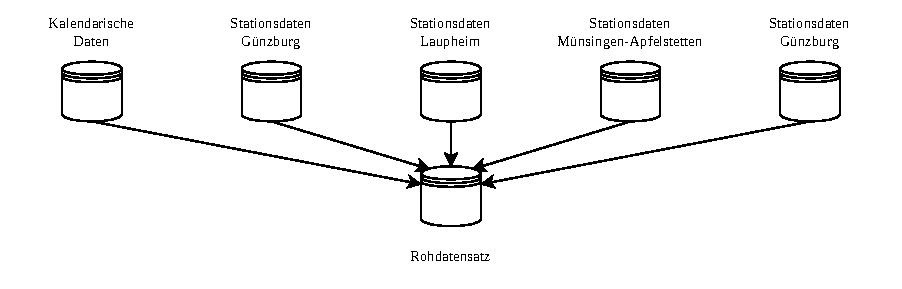
\includegraphics[]{./images/rohdatensatz.pdf}
		\caption{Zusammensetzung des Rohdatensatzes}
		\label{fig:rohdatensatz}
	\end{center}
\end{figure}
%%%%%BILD ENDE

\subsection{Reale Messdaten}
Die realen Messdaten werden vom Deutschen Wetterdienstes über einen Webserver kostenlos zur Verfügung gestellt. In dieser Arbeit sind die Daten in stündlicher Auflösung von vier Messtationen (Münsingen-Apfelstetten, Stötten, Günzburg und Laupheim) im Ulmer Umkreis zum Einsatz gekommen. Die genaue geographische Lage kann der Abbildung \ref{fig:map} entnommen werden. Der Deutsche Wetterdienst betreibt im Ulmer Umkreis zwar noch weitere Wetterstationen, jedoch messen diese die Windgeschwindigkeit und Windrichtung nicht. Insgesamt umfasst der Datensatz die Jahre \highlight{2008?} bis 2021. Davon sind jedoch \highlight{X\%} Datenlücken. Diese Lücken werden in Kapitel \ref{section:Datenlücken} genauer beleuchtet. 

%%%%%BILD ANFANG
\begin{figure}[tph]
	\begin{center}
		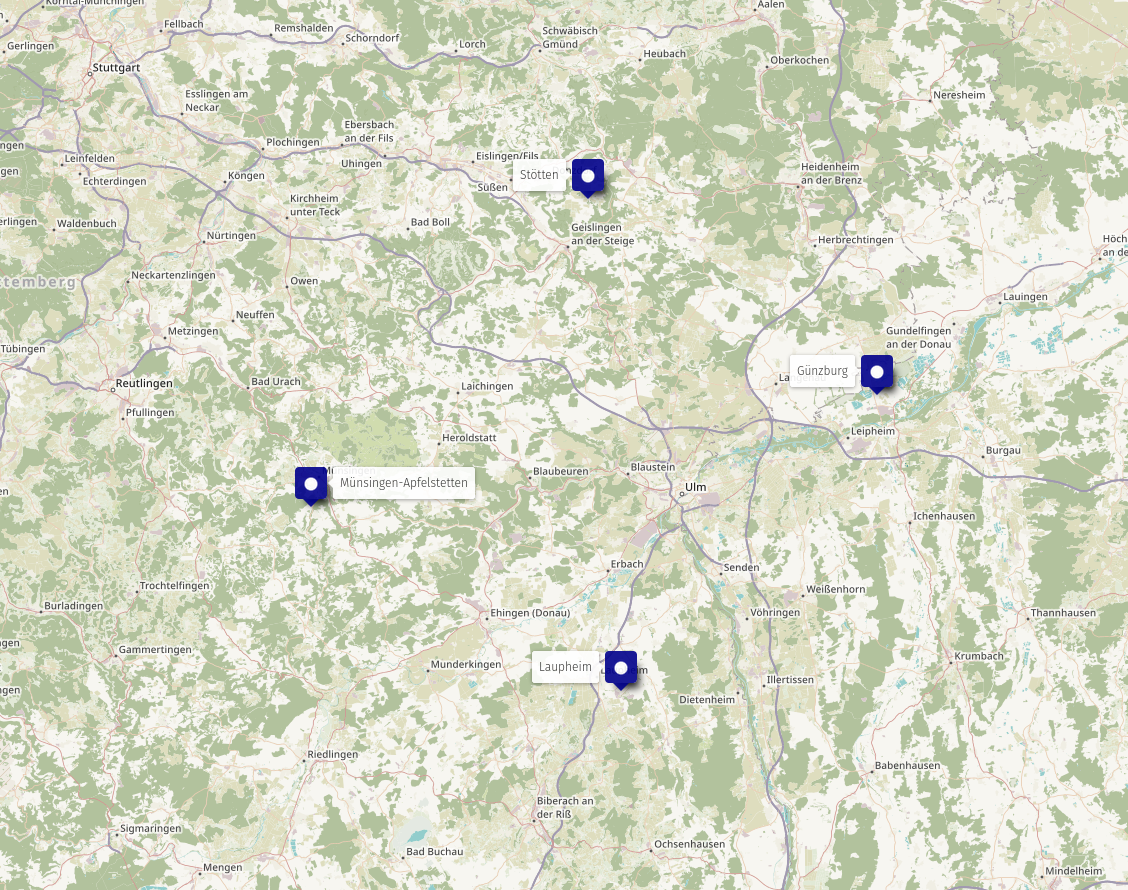
\includegraphics[width=\textwidth]{./images/map.png}
		\caption{Geographische Lage der Messstationen \cite{2021_OpenStreetMap-Contributors_UMap}}
		\label{fig:map}
	\end{center}
\end{figure}
%%%%%BILD ENDE

Zur Prognose der Windgeschwindigkeit und Windrichtung können neben deren selbst \highlight{(Satzbau?)} auch andere Messgrößen wie Sonnenscheindauer, Luftdruck, Temperatur und Luftfeuchtigkeit genutzt werden. Jedoch wird nicht jede dieser Größen an jeder Messstation bestimmt. Die folgende Tabelle \ref{tab:messgrößen} gibt einen detaillierteren Aufschluss über die tatsächlich gemessenen Größen.

%%%%%TABELLE ANFANG
\begin{table}[ht]
	\centering
	\caption{Gemessene Größen je Messstation \highlight{Auflösung der einzelnen Größen ergänzen. Wird referenziert!}}
	\begin{tabular}{|l|c|c|c|c|}
		\hline
        \rowcolor{color80}
		& \textbf{Münsingen-Apfelstetten} & \textbf{Stötten} & \textbf{Günzburg} & \textbf{Laupheim} \\\hline
		Windgeschwindigkeit & \cmark & \cmark & \cmark & \cmark \\\hline
		Windrichtung & \cmark & \cmark & \cmark & \cmark \\\hline
		Sonnenscheindauer & \cmark & \cmark & \xmark & \xmark \\\hline
		Luftdruck & \xmark & \cmark & \xmark & \cmark \\\hline
		Temperatur & \cmark & \cmark & \cmark & \cmark \\\hline
		Luftfeuchtigkeit & \cmark & \cmark & \cmark & \cmark \\\hline
	\end{tabular}
\label{tab:messgrößen}
\end{table}
%%%%%TABELLE ENDE

Um einen tieferen Einblick in das Verhalten des Windes an der jeweiligen Messstation zu erhalten, bieten sich Windrosen zur Visualisierung an. Dabei wird die Häufigkeit der Windgeschwindigkeit in Abhängigkeit der Windrichtung radial dargestellt. Der Abbildung \ref{fig:windroses} können die Windrosen für die vier ausgewählten Messstationen entnommen werden. Wie in den südlichen Regionen Deutschlands zu erwarten \highlight{satzbau?}, ist die vorherschende Windrichtung West bis Südwest. 

Bei detaillierter Analyse fällt jedoch auf, dass der Wind an der Messstationen Münsingen-Apfelstetten besonders bei Leichtwind sehr volatil ist. Der Grund hierfür könnte in der Tatsache begründet sein, dass sich die Messstation in einem flachen Tal mit Nord-Südlicher Ausrichtung befindet. Desweiteren lässt sich erkennen, dass unter den vier Messstationen in Stötten die stärksten Winde auftreten. 

%%%%%BILD ANFANG
\begin{figure}[tph]
	\begin{center}
		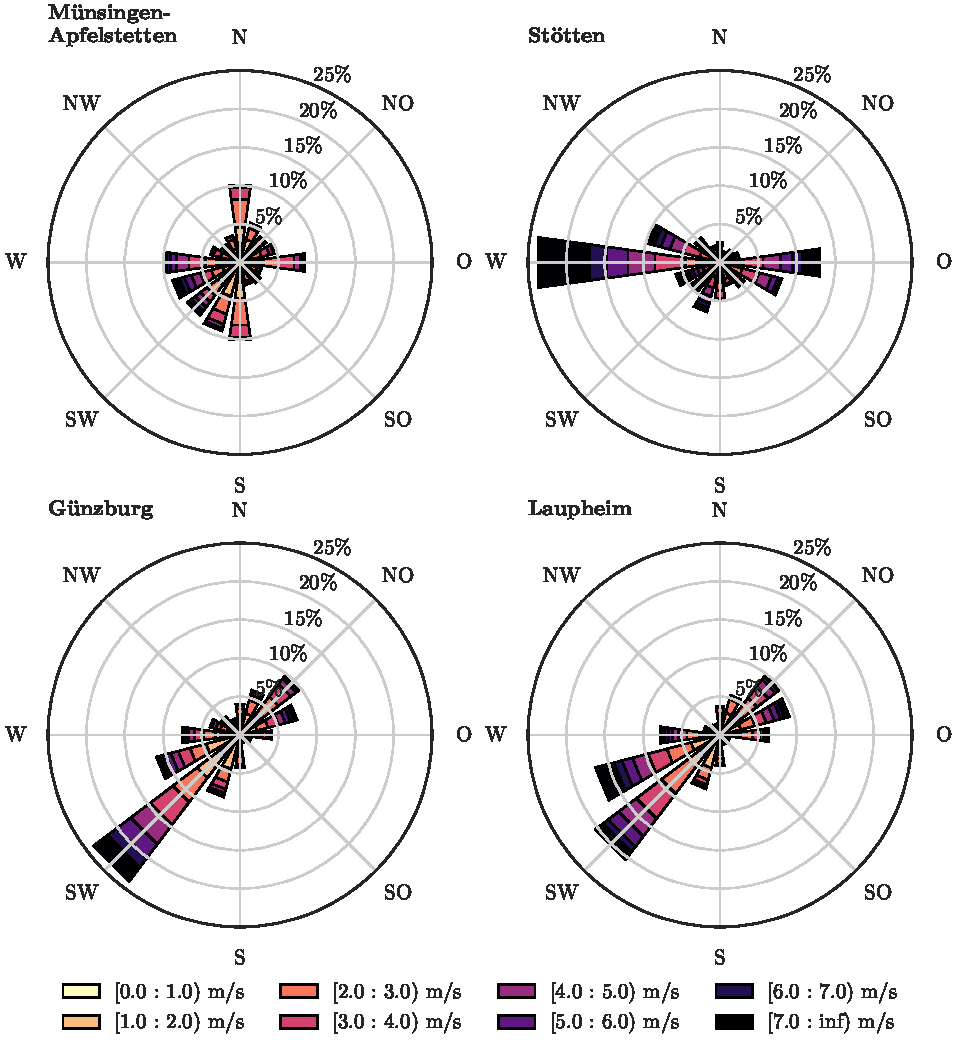
\includegraphics[]{./images/windroses.pdf}
		\caption{Windrosen der vier ausgewählten Messstationen}
		\label{fig:windroses}
	\end{center}
\end{figure}
%%%%%BILD ENDE

Im Folgenden wird versucht, die Windgeschwindigkeit \highlight{und Windrichtung?} für die Messstation in Günzburg \highlight{und Stötten?} zu prognostizieren. 

\highlight{Warum Günzburg? 1. Liegt östlich der anderen Stationen 2. Relativ klare Windrose}

\highlight{Warum Stötten? 1. Alle Messgrößen werden vorort gemessen 2. Stärkster Wind}

\subsection{Generierte Messdaten}\label{section:gen_daten}
Die Wetterlage in Deutschland weist wiederkehrende Trends innerhalb eines Tages und auch innerhalb eines Jahres auf. Offensichtlich ist es am Tag wärmer als in der Nacht und im Sommer wärmer als im Winter. Um diese Information für das Modell nutzbar zu machen, werden zusätzlich zu den gemessenen Daten zwei weitere Variablen eingeführt: \highlight{Warum Sinus? Weil zirkuläre Daten! 24h=0h! Oben gibts das Kapitel \ref{section:circ_data} in dem zirkuläre Daten erklärt werden, d.h. erwähnen!}

\begin{itemize}
	\item \textit{Kalendarischer Tageswert}\\
	Über die folgende Funktion wird die Stunde des Tages $HOD \in [0, \dots, 23]$ in einen Sinuswelle umgewandelt. Das Maximum wird um 12 Uhr, das Minimum um 0 Uhr erreicht. Abgebildet wird auf das Intervall $[0,1]$.
	\begin{equation}\label{eq:cal_day}
		cal_{day} = \frac{1}{2}\Big(\cos \big(\pi (\frac{HOD}{12}+ 1)\big) + 1 \Big)
	\end{equation}
	\item \textit{Kalendarischer Saisonalwert}\\
	Die folgende Funktion transformiert den Tag des Jahres $DOY \in [1, \dots, 365]$ in eine Sinuswelle. Schaltjahre werden nicht berücksichtigt. Außerdem wird die Stunde des Tages $HOD \in [0, \dots, 23]$ mit einbezogen. Diese spielt für den Funktionswert jedoch nur eine untergeordnete Rolle. Das Maximum wird am 1.Juli, das Minimum am 1.Januar erreicht. Die Funktion bildet ebenfalls auf das Intervall $[0,1]$ ab.
	\begin{equation}\label{eq:cal_seas}
		cal_{seas} = \frac{1}{2}\Big(\cos\big(\pi (\frac{DOY -1 + \frac{HOD}{24}}{\frac{365}{2}}+ 1)\big) + 1\Big)
	\end{equation}
	
\end{itemize}

\highlight{Eventuell erwähnen, das diese Formeln nicht optimal sind. Grund: Höchste Tagestemperatur i.A. nicht um 12 Uhr sondern um 13-14 Uhr, Höchste Jahrestemperatur i.A. nicht am 1.Juli sondern Mitte August. Außerdem ist z.B. $dal_{day}(HOD=6Uhr) = dal_{day}(HOD=18Uhr)$}

\subsection{Analyse der Datenbasis}
Der Korrekatinskoeffizient gibt Aufschluss darüber, ob zwischen zwei größen ein linearer Zusammenhang besteht. Er kann als Entscheidungshilfe zur Auswahl der Input-Größen für das neuronale Netz dienen. In Abbildung \ref{fig:corr} wird die Korrelation zwischen den Größen relative Luftfeuchte ($RH$), Sonnenscheindauer ($SD$), Temperatur ($T$), Windgeschwindigkeit ($v$), Windrichtung ($\varphi$) sowie die in Kapitel \ref{section:gen_daten} beschriebenen kalendarischen Daten $cal_{day}$ und $cal_{seas}$ dargestellt. 



Da die Größen Windstärke und \highlight{Windrichtung?} prognostiziert werden sollen, sind die Korrelationen zwischen dieser und anderer Größen natürlich von besonderem Interesse. Aus Abbildung \ref{fig:corr} lässt sich erkennen, dass der Luftdurck in einem Zusammenhang mit der Windgeschwindigkeit steht (Fällt $RH$ steigt $v$). Ebenso lässt sich aus der Korrelation zwischen Windgeschwindigkeit und der Temperatur bzw. dem kalendarischen Saisonalwert $cal_{seas}$ eine erhöhte Windgeschwindigkeit im Winter ablesen. Der kalendarische Tageswert $cal_{day}$ scheint jedoch nicht in einem linearen Zusammenhang mit der Windgeschwindigkeit zu stehen.

\bigskip
An dieser Stelle ist es wichtig zu erwähnen, dass der Korrelationskoeffizient nur einen linearen Zusammenhang zwischen zwei größen abbildet. Komplexere Zusammenhänge werden nicht erkannt \cite{2020_Ranjan_EstimatingNonlinearCorrelation}. Es ist also möglich, dass eine Größe für die Prognose wertvolle Information enthält, jedoch nicht mit der Windgeschwindigkeit korreliert.

%%%%%BILD ANFANG
\begin{figure}[tph]
	\begin{center}
		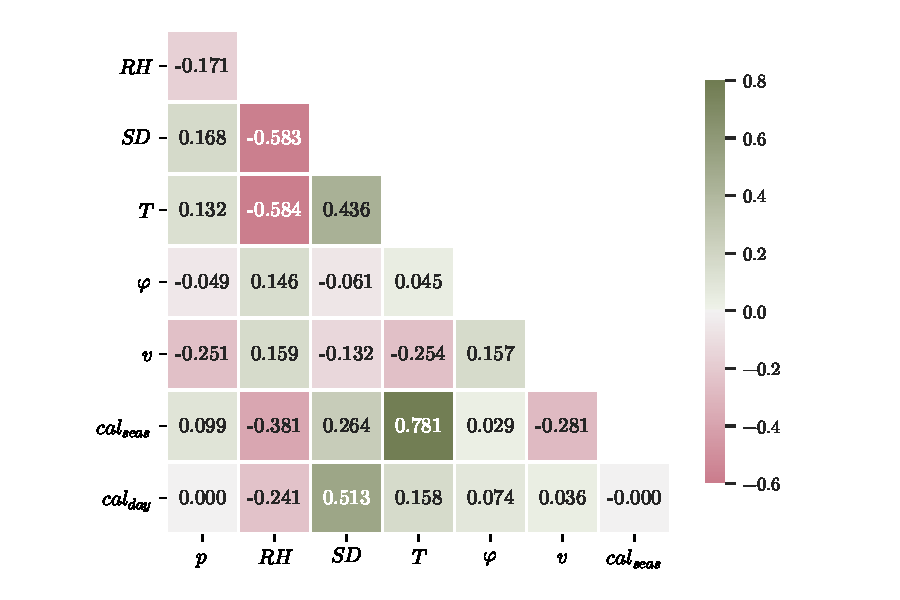
\includegraphics[]{./images/corr.pdf}
		\caption{Korrelationskoeffizienten für die Messdaten der Station in Stötten \highlight{(Ändern zu Günzburg, da diese prognostiziert wird)} sowie kalendarische Daten im Zeitraum 01.01.2016 bis 31.12.2020.}
		\label{fig:corr}
	\end{center}
\end{figure}
%%%%%BILD ENDE

\highlight{Grafikidee: Windgeschwindigkeit über Uhrzeit}

\section{Datenaufbereitung}\label{section:Datenaufbereitung}
Die Datenaufbereitung ist häufig eines der aufwendigeren Teile eines Machine-Learning Projektes. Daher wird in dieser Arbeit auf diesen Teil vertieft eingegangen. Abbildung \ref{fig:preprocessing} skizziert den Ablauf der Datenaufbereitung. Dabei werden die folgenden fünf Schritte durchlaufen, die in den nachfolgenden Kapiteln detaillierter beschrieben werden:

%%%%%BILD ANFANG
\begin{figure}[tph]
	\begin{center}
		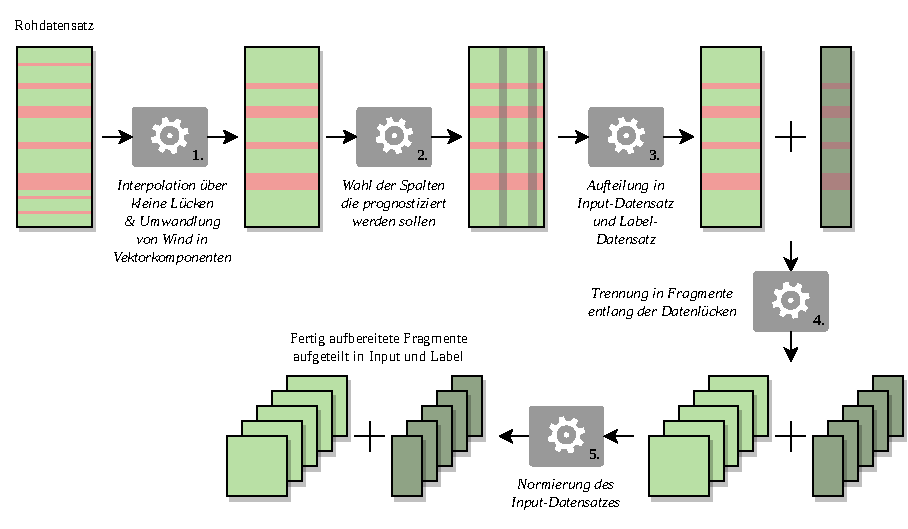
\includegraphics[]{./images/preprocessing.pdf}
		\caption{Ablauf der Datenaufbereitung. \highlight{Beschreiben, dass die grünroten Box der Datensatz ist}}
		\label{fig:preprocessing}
	\end{center}
\end{figure}
%%%%%BILD ENDE

\begin{enumerate}
	\item Im Rohdatensatz gibt es einige kürzere und längere Datenlücken (In Abb. \ref{fig:preprocessing} dargestellt als rote Segmente). Über kurze Datenlücken wird linear interpoliert. Außerdem werden die Winddaten von der polaren in eine kartesische Darstellung umgewandelt.
	\item Aus dem durch Schritt 1. generierten Datensatz werden die Spalten gewählt, die es zu prognostizieren gilt (In Abb. \ref{fig:preprocessing} dargestellt durch verdunkelte Spalten). In dieser Arbeit wird die Windgeschwindigkeit \highlight{(und Windgeschwindigkeit?)} einer Station gewählt.
	\item Der Datensatz wird nun in einen Inputdatensatz und einen Labeldatensatz (In Abb. \ref{fig:preprocessing} verdunkelt) aufgeteilt.
	\item Die verbleibenden längeren Datenlücken im Input- und Labeldatensatz werden \qm{herausgeschnitten}. Übrig bleiben Fragmentpaare, die keine Fehlstellen enthalten.
	\item Der Inputdatensatz (hellgrün) wird normiert. Dieser Schritt erleichtert das Training des neuronalen Netzes.
\end{enumerate}

\subsection{Interpolation über Datenlücken}\label{section:Datenlücken}
\highlight{Grafik wo und wie lange es im Datensatz Lücken gibt --> Heatmap}

\highlight{
	\begin{enumerate}
		\item Datenlücken für jede Messgröße seperat angeschaut
		\item Max Länge der Lücke über die noch interpoliert wird sind 4h
	\end{enumerate}
}
\subsection{Winddaten als Vektoren}
Die Windmessung erfolgt (von modernen Laser- oder Schallmessungen abgesehen) üblicher Weise mithilfe einens Schalenanemometers und einer Windfahne. Zu jedem Messzeitpunkt werden also zwei Werte aufgenommen. Die Windgeschwindigkeit $v$ wird in $m/s$ gemessen. Die Windrichtung $\varphi$ wird typischer Weise in Grad angegeben, es gilt also $\varphi \in [0,360)$. Norden wird dabei mit $\varphi_{north} = 0^\circ$ gewählt. Dieses $(v,\varphi)$-Tupel lässt sich als Polarkoordinate interpretieren. Jedoch tritt hier das in Kapitel \ref{section:circ_data} beschriebene Problem der zirkulären Daten auf, da $\varphi_{north} = 0^\circ = 360^\circ$ gilt.

Es gilt zu belegen, dass sich dieses Problem umgehen lässt, indem der Wind nicht in polaren sondern kartesischen Koordinaten dargestellt wird. Der Windvektor, der durch das $(v,\varphi)$-Tupel beschrieben ist, wird so in eine $v_x$ und eine $v_y$ Komponente zerlegt. Dieses Vorgehen ist in Abbildung \ref{fig:pol2cart} skizziert.

\highlight{Gleichung pol2cart?}

%%%%%BILD ANFANG
\begin{figure}[tph]
	\begin{center}
		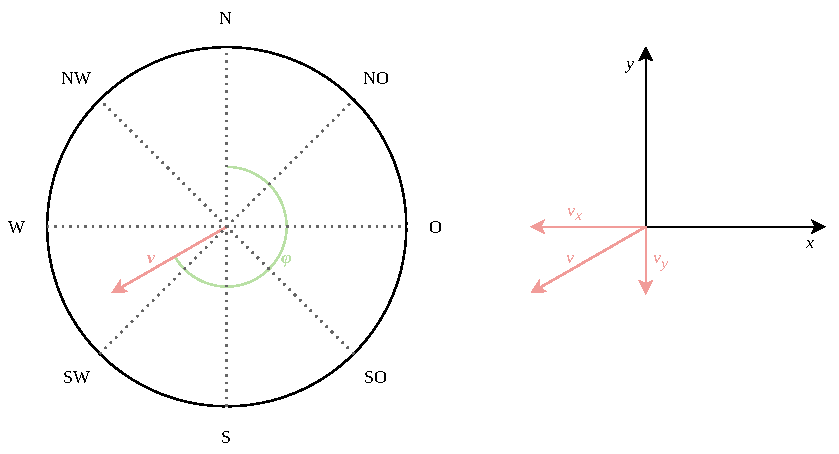
\includegraphics[scale = 1]{./images/pol2cart.pdf}
		\caption{Interpretation der Windgeschwindigkeit und Windrichtung als Vektorkomponenten}
		\label{fig:pol2cart}
	\end{center}
\end{figure}
%%%%%BILD ENDE

\highlight{Evtl erwähnen dass wenn diese Umwandlung genutzt wird, nach dem NN wieder zurück umgewandelt wird. d.h. $(v_x,v_y) \rightarrow (v,\varphi) \rightarrow(v_x,v_y)$}

Die hier beschriebene Umwandlung kann der Abbildung \ref{fig:pol2cart2} anhand realer Messdaten entnommen werden. Im oberen Teil ist die Häufigkeitsverteilung in $(v,\varphi)$-Form dargestellt. Die zirkuläre Eigenschaft $\varphi_{north} = 0^\circ = 360^\circ$ ist hier nicht sichtbar. Die Häufigkeitsverteilung für die umgewandelten Koordinaten in $(v_x,v_y)$-Form hingegen ist klar um den Ursprung verteilt. Hier lässt sich die zirkuläre Eigenschaft gut erkennen. Das strahlenartige Muster erklärt sich durch die diskrete Angabe der Windrichtung in $10^\circ$ Schritten. Bei einer feineren Auflösung wäre die Verteilung weniger verzerrt.

%%%%%BILD ANFANG
\begin{figure}[tph]
	\begin{center}
		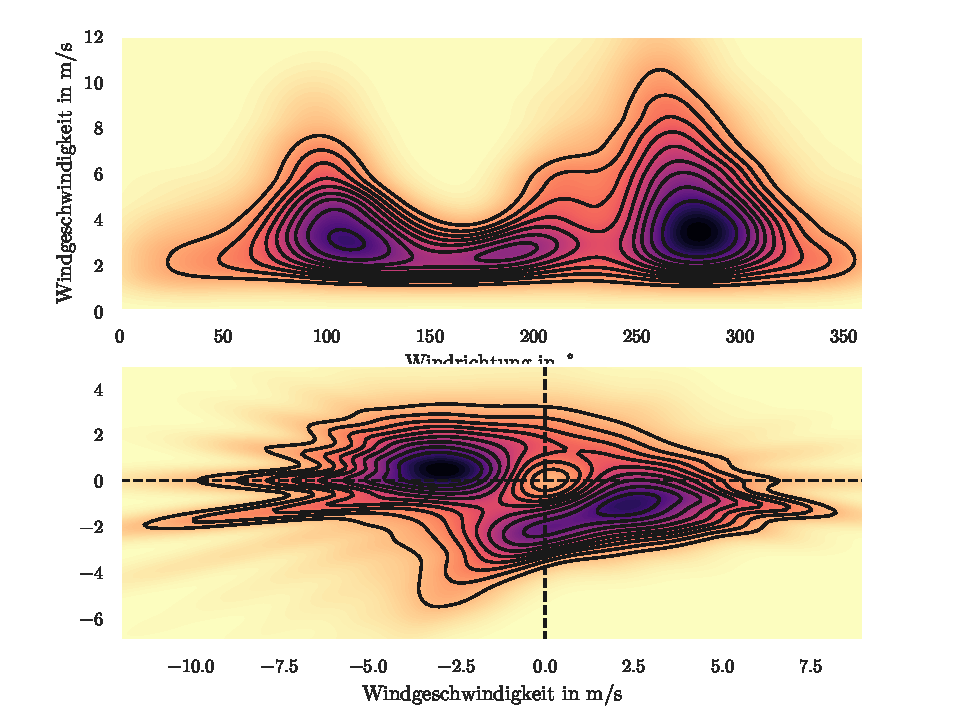
\includegraphics[scale = 1]{./images/pol2cart_visualize.pdf}
		\caption{Verteilung des Windes bei $(v,\varphi)$ bzw. $(v_x,v_y)$-Interpretation für die Messtation Ulm-Mähringen \highlight{(Ändern zu Günzburg, da diese prognostiziert wird)} im Zeitraum 01.2016 bis 03.2021 \highlight{FEHLER IN GRAFIK: x-Label Oben wird überdeckt}}
		\label{fig:pol2cart2}
	\end{center}
\end{figure}
%%%%%BILD ENDE

\subsection{Aufteilung in Input- und Labeldatensatz}
\highlight{
	\begin{itemize}
		\item Warum teilen?
		\item Größen konkret nennen
		\item Mit Grafik erklären
	\end{itemize}
}

\subsection{Normierung}

\highlight{Erklärung, warum Normierung nötig ist. Tabelle überdenken.}

%%%%%TABELLE ANFANG
\begin{table}[ht]
	\centering
	\caption{Normalisierung der Eingabedaten}
	\begin{tabular}{|c|c|c|c|c|c|c|c|}
		\hline
		\rowcolor{color80}
		\textbf{$X$} & \textbf{$w_x$} & \textbf{$w_y$} & \textbf{$p$} & \textbf{$T$} & \textbf{$RH$} & \textbf{$cal_{day}$} & \textbf{$cal_{seas}$} \\ \hline
		Einheit $X$ & $m/s$ & $m/s$ & $hPa$ & $^\circ C$ & \% & $1$ & $1$ \\ \hline
		$min(X)$       & $-22.1$ & $-13.7$ & $975.2$ & $-19.1$ & $10$ & $0$ & $0$ \\ \hline
		$max(X)$       & $13.5$ & $9.7$ & $1047.3$ & $34.4$ & $100$ & $1$ & $1$ \\ \hline
		$min(norm(X))$ & $-1$ & $-1$ & $0$ & $0$ & $0$ & $-$ & $-$ \\ \hline
		$max(norm(X))$ & $1$ & $1$ & $1$ & $1$ & $1$ & $-$ & $-$ \\ \hline
	\end{tabular}
\label{tab:normalisierung}
\end{table}
%%%%%TABELLE ENDE

\section{Generierung der Trainingsbeispiele}
Nachdem die Rohdaten aufgearbeitet worden sind, gilt es nun tatsächliche Trainingsbeispiele (Samples) zu generieren. Dieser Prozess wird in Abbildung \ref{fig:sampling} dargestellt, wobei die Grafik als Fortsetzung von Abbildung \ref{fig:preprocessing} verstanden werden kann. Das Ziel des Samplings ist die Generierung eins Pools aus Trainingsbeispielen, womit das neuronale Netz angelernt werden kann.

Zunächst müssen die Größen der Moving-Windows (siehe Abb. \ref{fig:sampling})festgelegt werden. Bei den Inputdaten gibt die Größe $n$ des Moving-Windows an, wieviele historische Zeitschritte für die Prognose genutzt werden. Das heißt, bei einer Prognose zum Zeitpunkt $t_0$ werden die Daten zu den Zeitpunkten $t_{n-1}, \dots, t_0$ als Inputdaten verwendet. Die Größe $m$ des Moving-Window auf den Labeldaten gibt den Prognosehorizont an. Das Ziel ist es also bei einer Prognose zum Zeitpunkt $t_0$ die Windgeschwindigkeiten \highlight{(und Windrichtungen?)} zu den Zeitpunkten $t_1, \dots, t_m$ vorherzusagen.

Das Ergebnis der Datenaufbereitung, beschrieben im Kapitel \ref{section:Datenaufbereitung}, sind datenlückenfreie Fragmentpaare. Ein solches Fragmentpaar besteht aus einem Input- und einem Labeldatensatz. Darüber werden nun die im vorherigen Schritt definierten Moving-Windows \qm{geschoben}. Die Schrittweite wird dabei kleinstmöglich gewählt, so entstehen am meisten Samples. Das Sampling wird auf jedem Fragmentpaar angewandt.

%%%%%BILD ANFANG
\begin{figure}[tph]
	\begin{center}
		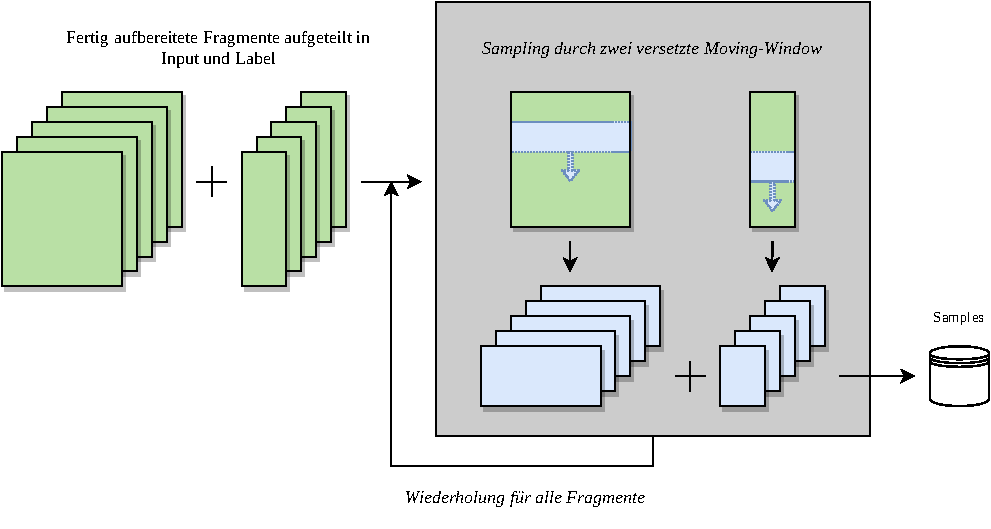
\includegraphics[]{./images/sampling.pdf}
		\caption{\highlight{{TODO}}}
		\label{fig:sampling}
	\end{center}
\end{figure}
%%%%%BILD ENDE

\highlight{
	An dieser Stelle feht noch, dass die Samples in drei Teile getrennt werden:
	\begin{itemize}
		\item Warum trennen?
		\item Aufteilung in Trainings (65\%), Validierungs(30\%) und Testdaten (5\%)
		\item Wieviele Samples haben wir?
	\end{itemize}
}

\section{Benchmarkmodell}
\highlight{Hier ist Platz für alles, was mit der implementierung des Vergleichsmodells zu tun hat. 
alles bis auf Ergebnisse}

\section{Entwicklung und Trainieren des Neuronalen Netzes}
\highlight{Hier ist Platz für alles, was mit der implementierung des eigentlichen Modells zu tun hat. 
Infos zu den Layers, zum Trainingsvorgang, Das mit den Decision Trees zur Auswahl der besten Paramter, 
alles bis auf Ergebnisse}

\subsection{Festlegung der Modellarchitektur \highlight{(Arbeitstitel)}}
\highlight{Begründen aus welchen Gründen wir uns für diese drei Methoden entschieden haben 
(RNNseq2seq, RNNseq2vec, DNN) z.B. Datengrundlage, Zeitaspekt, bla; 
Tabelele: Welche Lossfunktion, Metric, Prognosehorizont, Historie, tatsächliche Architektur (Schichten, Neuronen), 
welche Regularisierung + dazu immer etwas schreiben }

\subsection{Trainingsphase}
\highlight{Random search über Konfigurationen aus Tabelele und daraus optimales NN, hierüber schreiben; 
optionale Grafik über Fehler, Loss, und so}

\section{Ergebnisse}
\highlight{Hier nur die Ergebnisse zeigen und nüchtern darauf eingehen. Diskussion kommt ein Kapitel später. Einige Grafiken.}

%%%%%%%%%%%%%%%%%%%%%%%%%%%%%%%%%%%%%%%%%%%%%%%%%%%%%%%%%%%%%%%%%%%%%%%
%                                                                     %
%                                                                     %
%                                                                     %
%                               KAPITEL                               %
%                                                                     %
%                                                                     %
%                                                                     %
%%%%%%%%%%%%%%%%%%%%%%%%%%%%%%%%%%%%%%%%%%%%%%%%%%%%%%%%%%%%%%%%%%%%%%%

\chapter{Diskussion und Ausblick}
\highlight{Oben gezeigten Ergebnisse werden verglichen und die Ergebnisse anhand von Fehlermaß und Vergleich mit anderem Ansatz diskutiert ;
Später noch Ausblick bla}

\section{Diskussion der Ergebnisse}
\highlight{Was auch immer wir herausbekommen. In Kontext setzen. War unser Modell vergleichsweise gut? Hier vll auch 
Diskussion über Unterschied zwischen eine und mehrere Wetterstationsdaten.}

\subsection{Vergleich der entwickelten Modelle}
\highlight{Fehler (RMSE, MAE) anschauen und interpretieren der unterschiedlichen Netze; 
Fehler pro Windgeschwindigkeit; Fehler über Prognosehorizont}

\subsection{Einfluss kartesischer Winddaten}
\highlight{Vergleich kartesisch und polar am besten Modell}, wieder auf Grafik oben eingehen

\subsection{Einordnung in existierenden Prognosemodellen \highlight{(Arbeitstitel)}}
\highlight{entweder SARIMA oder ein anderes Netz aus Paper (zB Amerika oder so) verwenden und grob vergleichen der Fehler und erklären, dass
 Klima ähnlich und deswegen eher vergleichbar, aber nicht absolute Sicherheit!!! (Geht über Umfang der arbeit hinaus)}

\section{Weiterentwicklung des Modells}
\highlight{Das ist der Ausblick. Was könnte man noch tolles anstellen wo wir aber keine Zeit mehr für hatten? Idee Ensemble-Modell, andere Daten 
verwenden, um Modell besser mit anderem bestehendem zu Vergleichen, Satellitendaten einbinden, weitere Modelle untereinander vergleichen mit Ulmer Klimadaten}

Ideen, mit dem man das Modell / die Ergebnisse verbassern kann:

\begin{enumerate}
	\item Andere Stationsdaten mit weniger volatier Windgeschwindigkeit (d.h. Daten am Mehr)
\end{enumerate}
%%%%%%%%%%%%%%%%%%%%%%%%%%%%%%%%%%%%%%%%%%%%%%%%%%%%%%%%%%%%%%%%%%%%%%%
%                                                                     %
%                                                                     %
%                                                                     %
%                               KAPITEL                               %
%                                                                     %
%                                                                     %
%                                                                     %
%%%%%%%%%%%%%%%%%%%%%%%%%%%%%%%%%%%%%%%%%%%%%%%%%%%%%%%%%%%%%%%%%%%%%%%
\chapter{Test und Wissen}

\section{Tabelle}
%%%%%TABELLE ANFANG
\begin{table}[ht]
	\centering
	\caption{Das hier ist eine Testtabelle, man beachte die gezwungene Breite in der rechten Spalte. Lässt sich einfach durch den Befehl C\{5cm\} erzeugen.}
	\begin{tabular}{|l|C{5cm}|}
		\hline
        \rowcolor{color80}
		\textbf{Erste Zelle}&\textbf{Ein Header}\\
		\hline
		Moin: & Zusammen\\\hline
		leer:&\\\hline
		Moin: & Zusammen\\\hline
		leer:&\\\hline
	\end{tabular}
\label{tab:testtabelle}
\end{table}
%%%%%TABELLE ENDE

%%%%%LANGTABELLE ANFANG
\begin{longtable}{|L{3.6cm}|L{6cm}|L{6cm}|}
	\caption{Finale Merkmale}\label{tab:longtable}\\
    % Definition des Tabellenkopfes auf der ersten Seite
	\hline
    \rowcolor{color80}
	\textbf{Abkürzung}&\textbf{Englisch}&\textbf{Deutsch}\\
	\hline
	\endfirsthead % Erster Kopf zu Ende
	% Definition des Tabellenkopfes auf den folgenden Seiten
	\hline
	\rowcolor{color80}
	\textbf{Abkürzung}&\textbf{Englisch}&\textbf{Deutsch}\\
	\hline
	\endhead % Zweiter Kopf ist zu Ende
    \hline
    \endfoot
    \hline
    \endlastfoot
	% Ab hier kommt der Inhalt der Tabelle
	$test_{\mathrm{abk}}$&ein sehr sehr sehr langertextmit langen wörternein sehr sehr sehr langertextmit langen wörternein sehr sehr sehr langertextmit langen wörternein sehr sehr sehr langertextmit langen wörternein sehr sehr sehr langertextmit langen wörtern&Einzeilig\\
	Z&5&as\\\hline
	A&1&91\\\hline
	B&2&97\\\hline
	Z&5&as\\\hline
	A&1&91\\\hline
	B&2&97\\\hline
	A&1&91\\\hline
	B&2&97\\\hline
	Z&5&as\\\hline
	A&1&91\\\hline
	B&2&97\\\hline
    Z&5&as\\\hline
	A&1&91\\\hline
	B&2&97\\\hline
	Z&5&as\\\hline
	A&1&91\\\hline
	B&2&97\\\hline
    Z&5&as\\\hline
	A&1&91\\\hline
	B&2&97\\\hline
	Z&5&as\\\hline
	A&1&91\\\hline
	B&2&97\\\hline
    Z&5&as\\\hline
	A&1&91\\\hline
	B&2&97\\\hline
	Z&5&as\\\hline
	A&1&91\\\hline
	B&2&97\\\hline
    Z&5&as\\\hline
	A&1&91\\\hline
	B&2&97\\\hline
	Z&5&as\\\hline
	A&1&91\\\hline
	B&2&97\\\hline
    Z&5&as\\\hline
	A&1&91\\\hline
	B&2&97\\\hline
	Z&5&as\\\hline
	A&1&91\\\hline
	B&2&97\\\hline
	Z&5&as\\\hline
	A&1&91\\\hline
	B&2&97\\\hline
	Z&5&as\\\hline
	A&1&91\\\hline
	B&2&97\\\hline
	Z&5&KEINE hline AM SCHLUSS!!!\\
\end{longtable}
%%%%%LANGTABELLE ENDE

\section{Bild}

%%%%%BILD ANFANG
\begin{figure}[tph]
	\begin{center}
		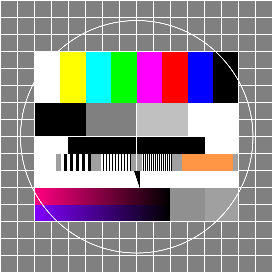
\includegraphics[scale = 1]{./images/0_testbild.png}
		\caption{TEST Hier ist ein wunderschönes Testbild zu erkennen, und das hier ist ein wunderschönes Testbild zu erkennen, und das hier ist ein wunderschönes Testbild zu erkennen, und das hier ist ein wunderschönes Testbild zu erkennen, und das hier ist ein wunderschönes Testbild zu erkennen, und das hier ist ein wunderschönes Testbild zu erkennen, und das hier ist ein}
		\label{fig:testbild}
	\end{center}
\end{figure}
%%%%%BILD ENDE

%%%%%DOPPELBILD ANFANG
\begin{figure}
	\centering
	\begin{minipage}[b]{.4\linewidth} % [b] => Ausrichtung an \caption
		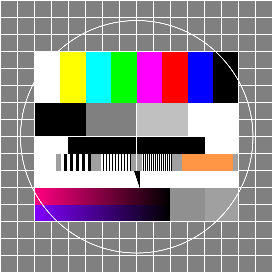
\includegraphics[width=\linewidth]{./images/0_testbild.png}
		\caption{Beschreibung und so}
		\label{fig:testbild_klein_links}
	\end{minipage}
	\hspace{.1\linewidth}% Abstand zwischen Bilder
	\begin{minipage}[b]{.4\linewidth} % [b] => Ausrichtung an \caption
		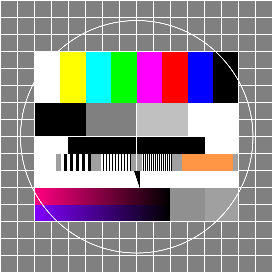
\includegraphics[width=\linewidth]{./images/0_testbild.png}
		\caption{Zweite Beschreibung}
		\label{fig:testbild_klein_rechts}
	\end{minipage}
\caption*{Hier steht eine etwas längere Bildunterschrift, die dieses Doppelbild beschreibt. Zu sehen sind weder Land noch Wasser, das macht bei Testbildern aber nix.}
\end{figure}
%%%%%DOPPELBILD ENDE

\section{Formeln}

Aufpassen, hier kommt jetzt eine einfache Testformel hin:

\begin{equation}
\label{eq:1}
x=10
\end{equation}

Diese Formel \autoref{eq:1} kann auch referenziert werden.

\begin{equation}
x=Ma_{\mathrm{blabla}} \cdot y
\end{equation}

\section{Zitate}

Um Bib zu kompilieren, einmal F8 drücken.

Bild \autoref{fig:testbild} referenzieren.
%Auch ein Autorname \citeauthor{ernstGrundkursInformatikGrundlagen2015} oder ein Jahr geht \citeyear{ernstGrundkursInformatikGrundlagen2015}

%%%%%%%%%%%%%%%%%%%%%%%%%%%%%%%%%%%%%%%%%%%%%%%%%%%%%%%%%%%%%%%%%%%%%%%
%                                                                     %
%                                                                     %
%                                                                     %
%                               KAPITEL                               %
%                                                                     %
%                                                                     %
%                                                                     %
%%%%%%%%%%%%%%%%%%%%%%%%%%%%%%%%%%%%%%%%%%%%%%%%%%%%%%%%%%%%%%%%%%%%%%%
\printbibliography[title=Literaturverzeichnis]
\end{document}